\section{Models and training}\label{section:models}

This study uses three different model architectures: ResNet 18 \cite{he2015deep}, DenseNet 121 \cite{huang2017densely} and EfficientNet B0 \cite{tan2019efficientnet}. These architectures were selected base on popularity in the data science community and  their availability in popular frameworks. Each model was first pretrained on the ImageNet dataset \cite{imagenet2009}, and fully connected layers from the top of the architecture were removed. There were no further changes to the original structures. On top of the model, a single fully-connected layer was added with the output size matching the number of classes in the particular dataset used for fine-tuning. Fine-tuning is done using Stochastic Gradient Descent (SGD) with momentum \cite{rumelhart1986learning} and Cross-Entropy loss function. Each model was trained for 15 epochs with a decrease of the learning rate (from \textit{0.001} to \textit{0.0001}) after the 7th epoch. Each architecture was trained on every available dataset and every training fraction split of that dataset (train dataset splitting described in section \ref{section:datasets}). In total, $75$ different models were trained for the purpose of the experiments.

\begin{figure}[h]
  \centering
 \begin{subfigure}{.45\textwidth}
    \centering
    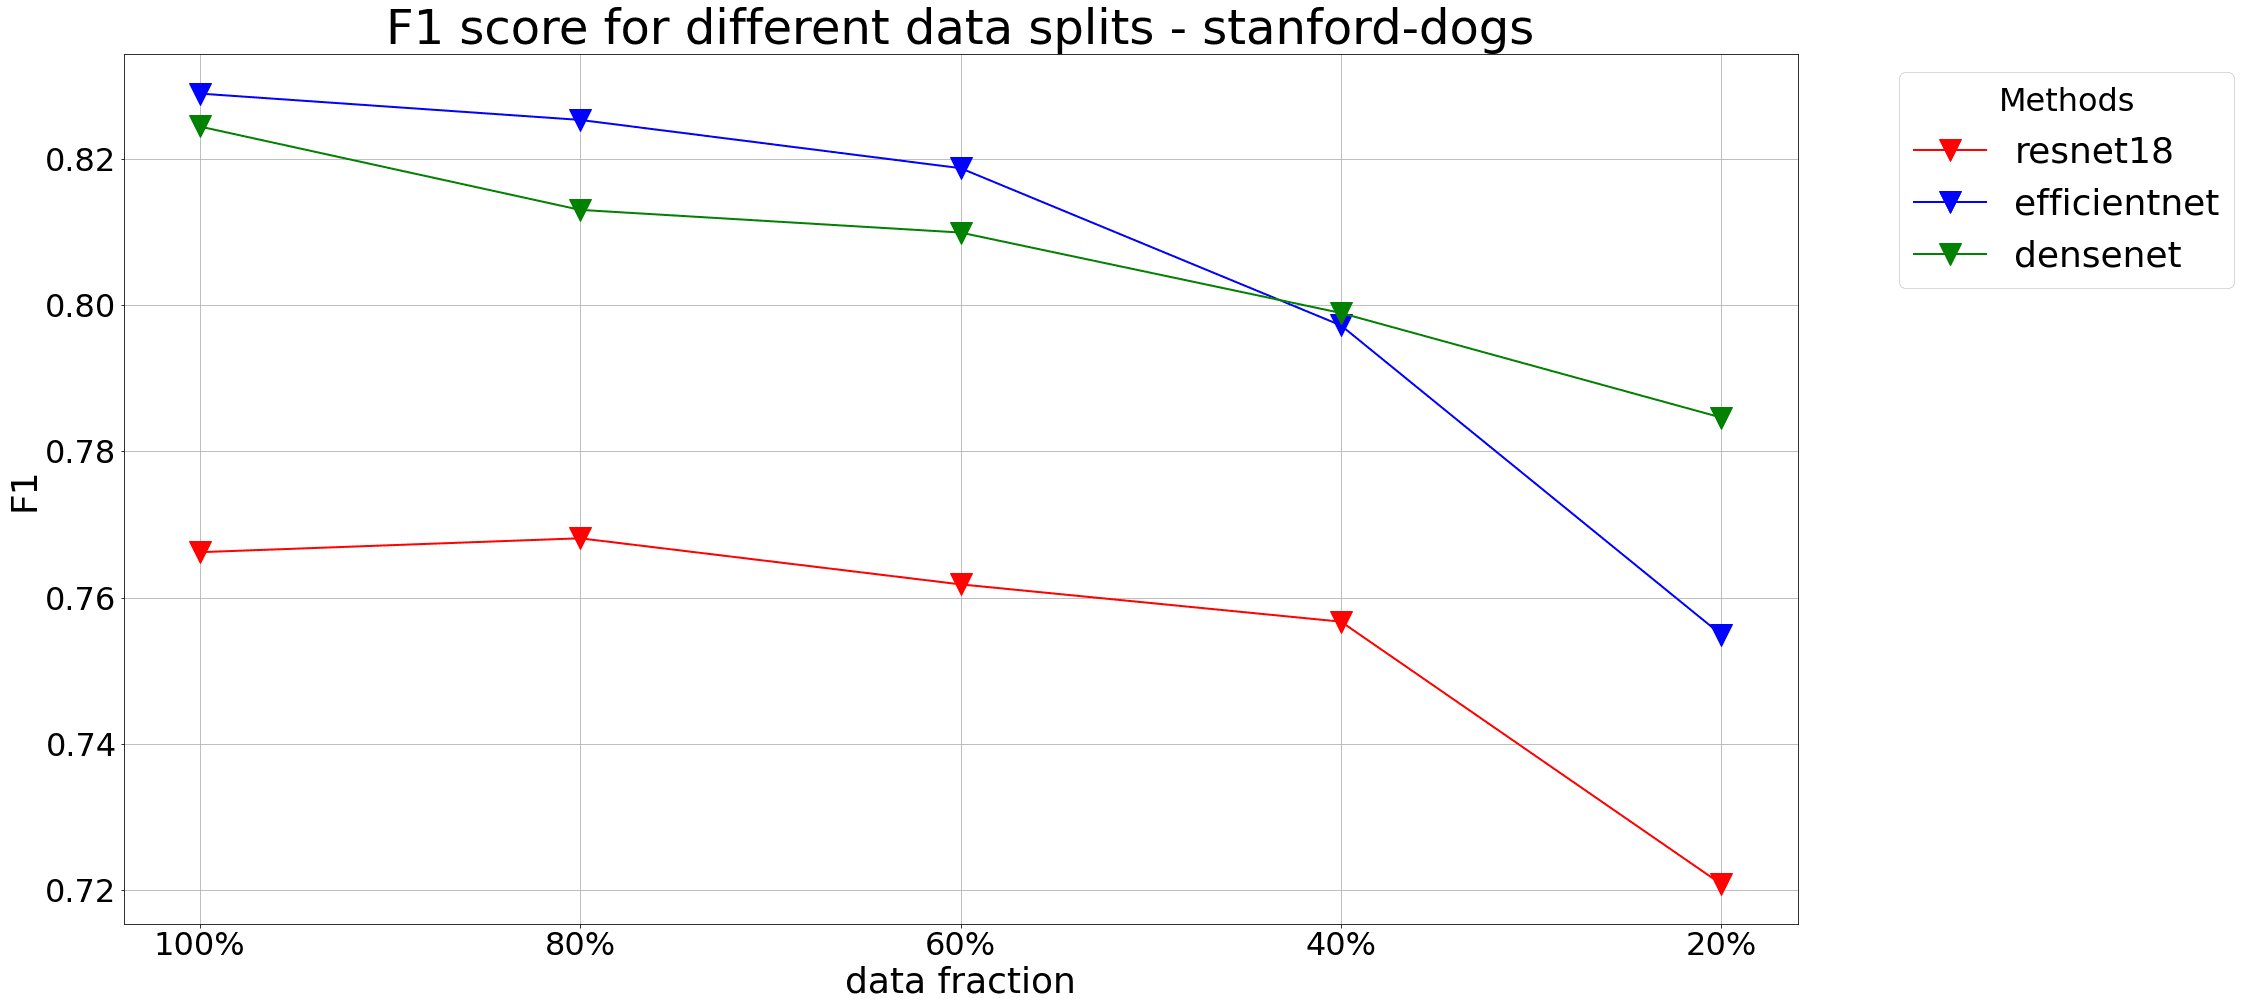
\includegraphics[width=\textwidth]{experiments/models/stanford-dogs-f1.png}
    \caption{Stanford Dogs dataset, F1 scores}\label{fig:model-scores-dogs}
\end{subfigure}
 \begin{subfigure}{.45\textwidth}
    \centering
    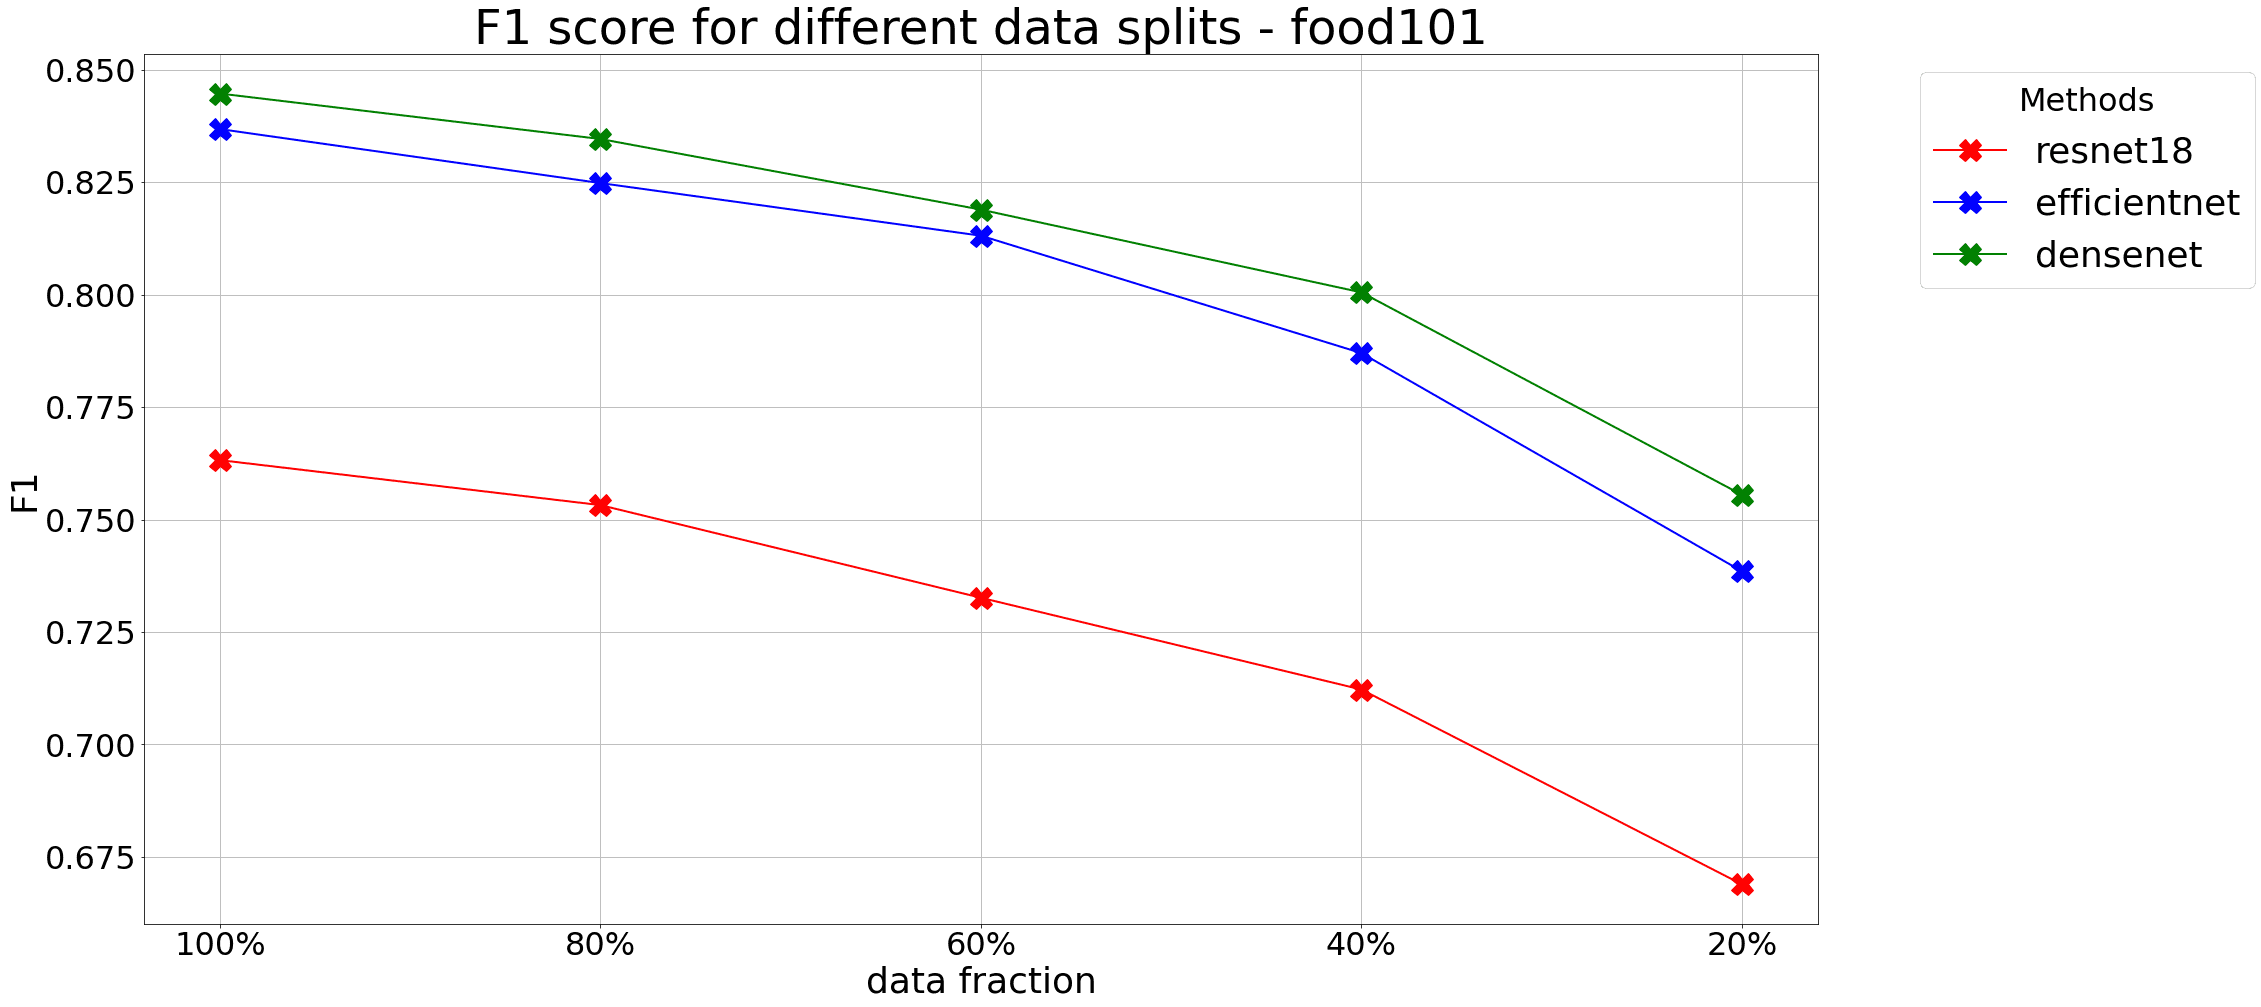
\includegraphics[width=\textwidth]{experiments/models/food101-f1.png}
    \caption{Food 101 dataset, F1 scores}\label{fig:model-scores-food101}
\end{subfigure}
 \begin{subfigure}{.45\textwidth}
    \centering
    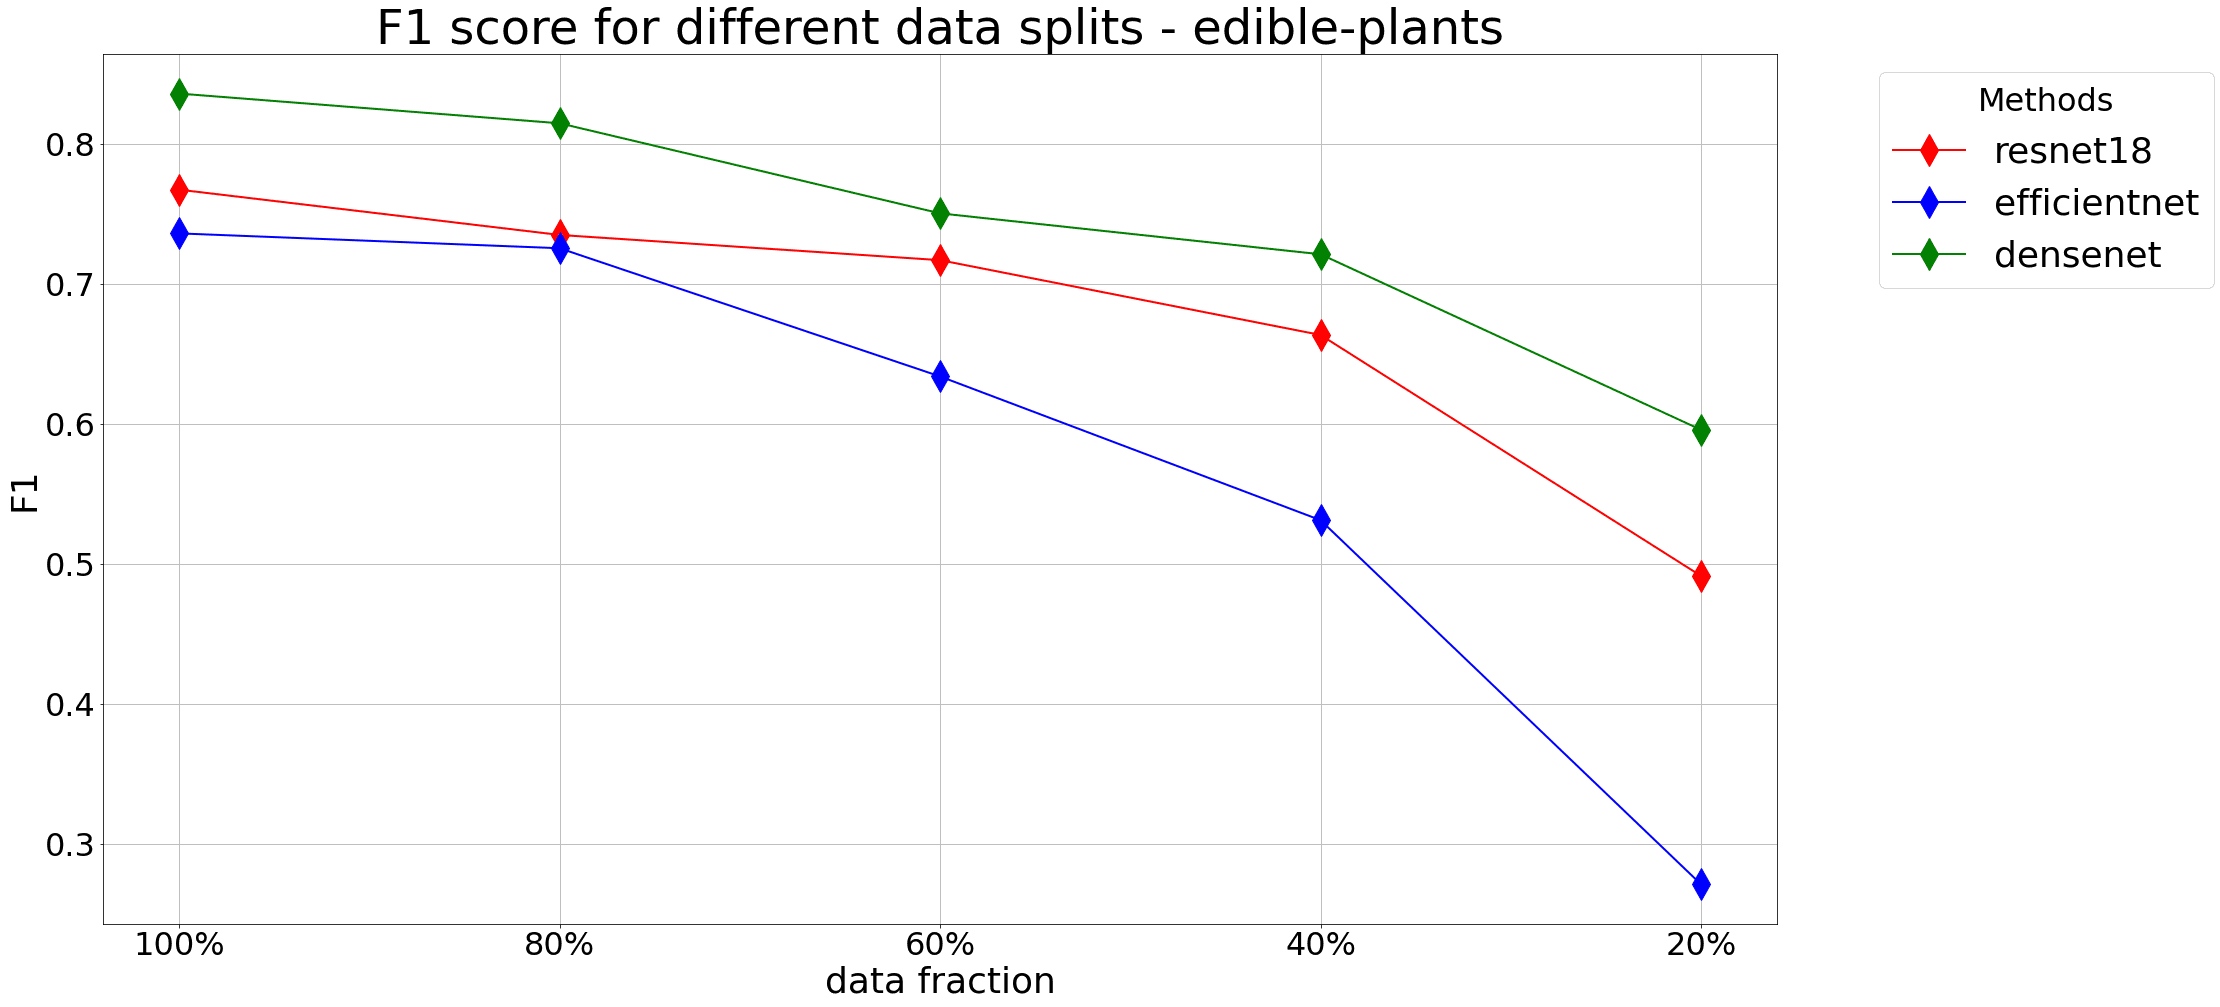
\includegraphics[width=\textwidth]{experiments/models/edible-plants-f1.png}
    \caption{Edible wild plants dataset, F1 scores}\label{fig:model-scores-edible-plants}
\end{subfigure}
 \begin{subfigure}{.45\textwidth}
    \centering
    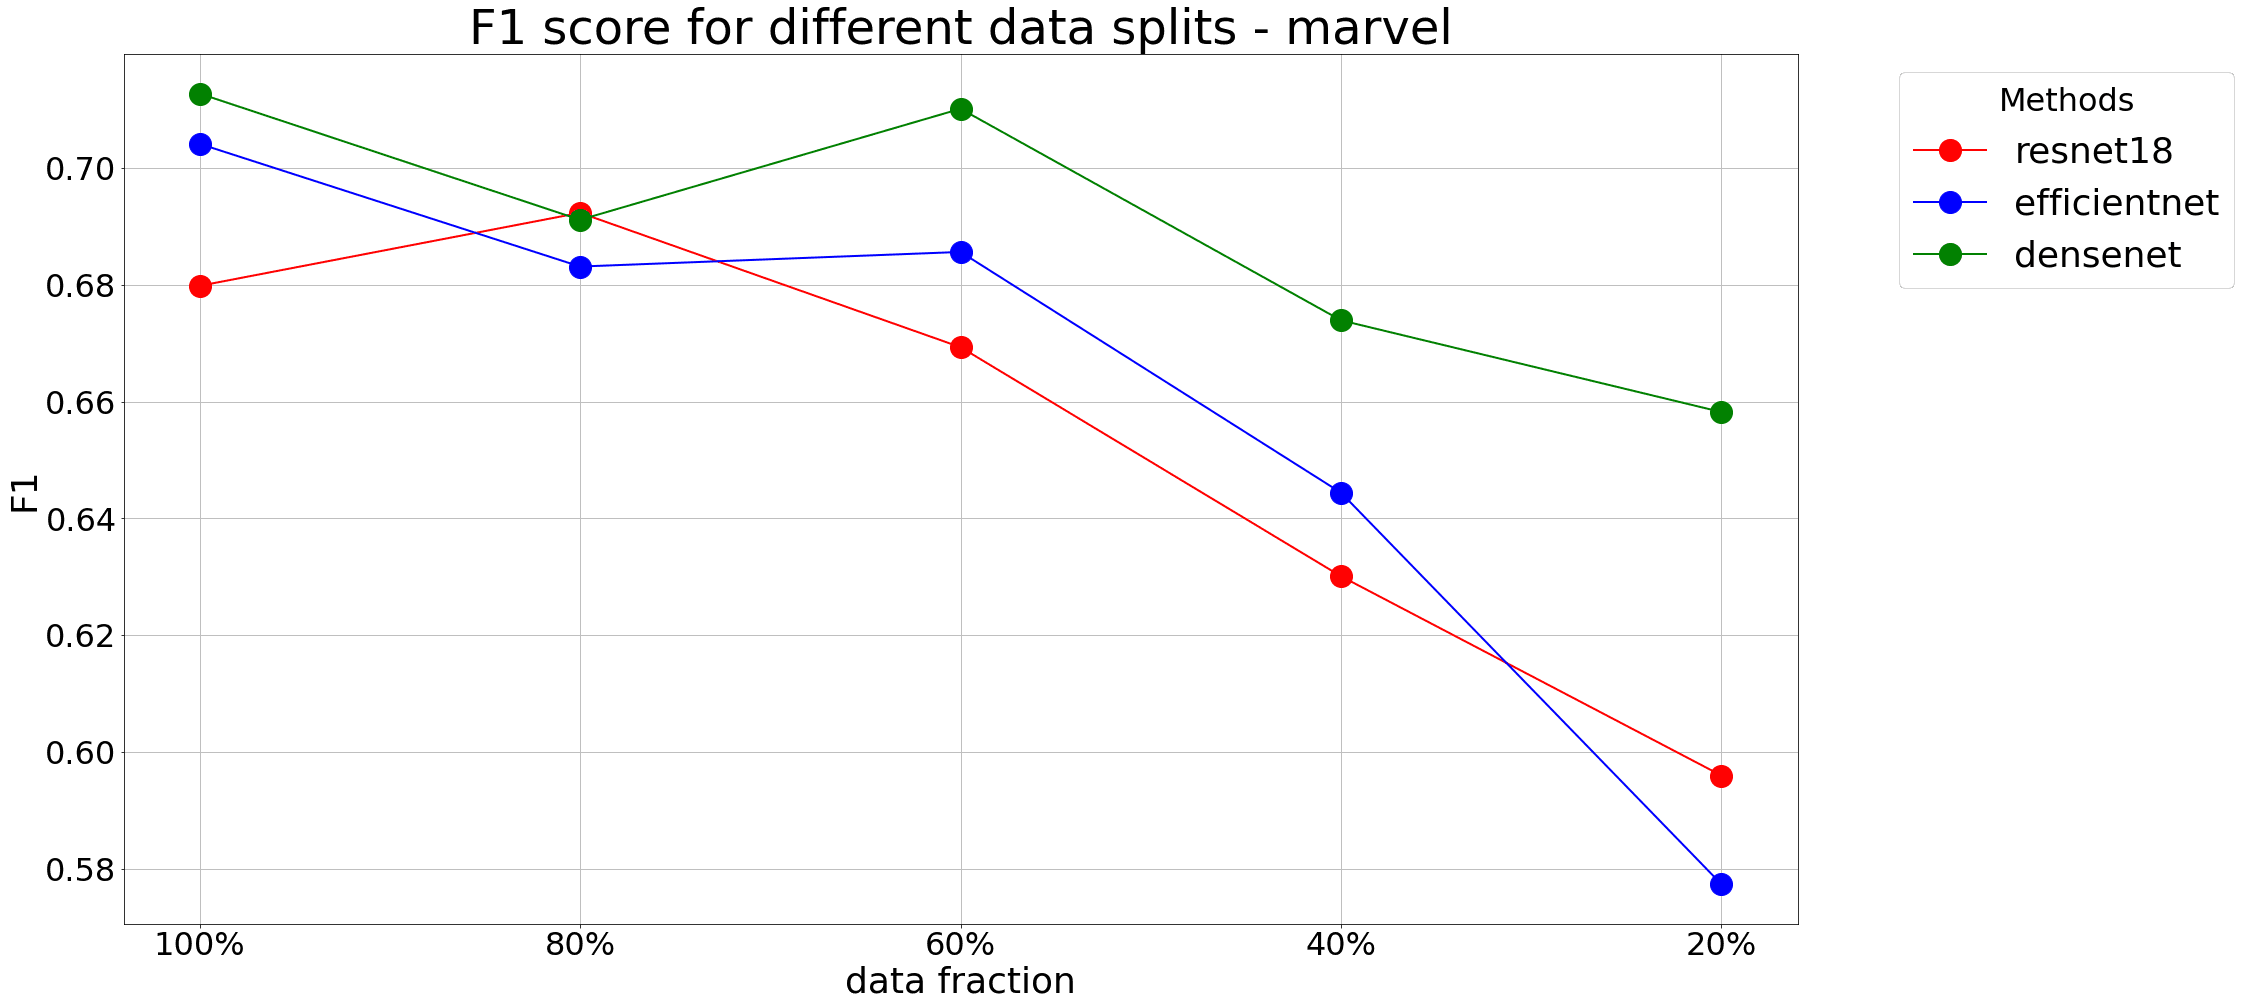
\includegraphics[width=\textwidth]{experiments/models/marvel-f1.png}
    \caption{Marvel dataset, F1 scores}\label{fig:model-scores-marvel}
\end{subfigure}
 \begin{subfigure}{.45\textwidth}
    \centering
    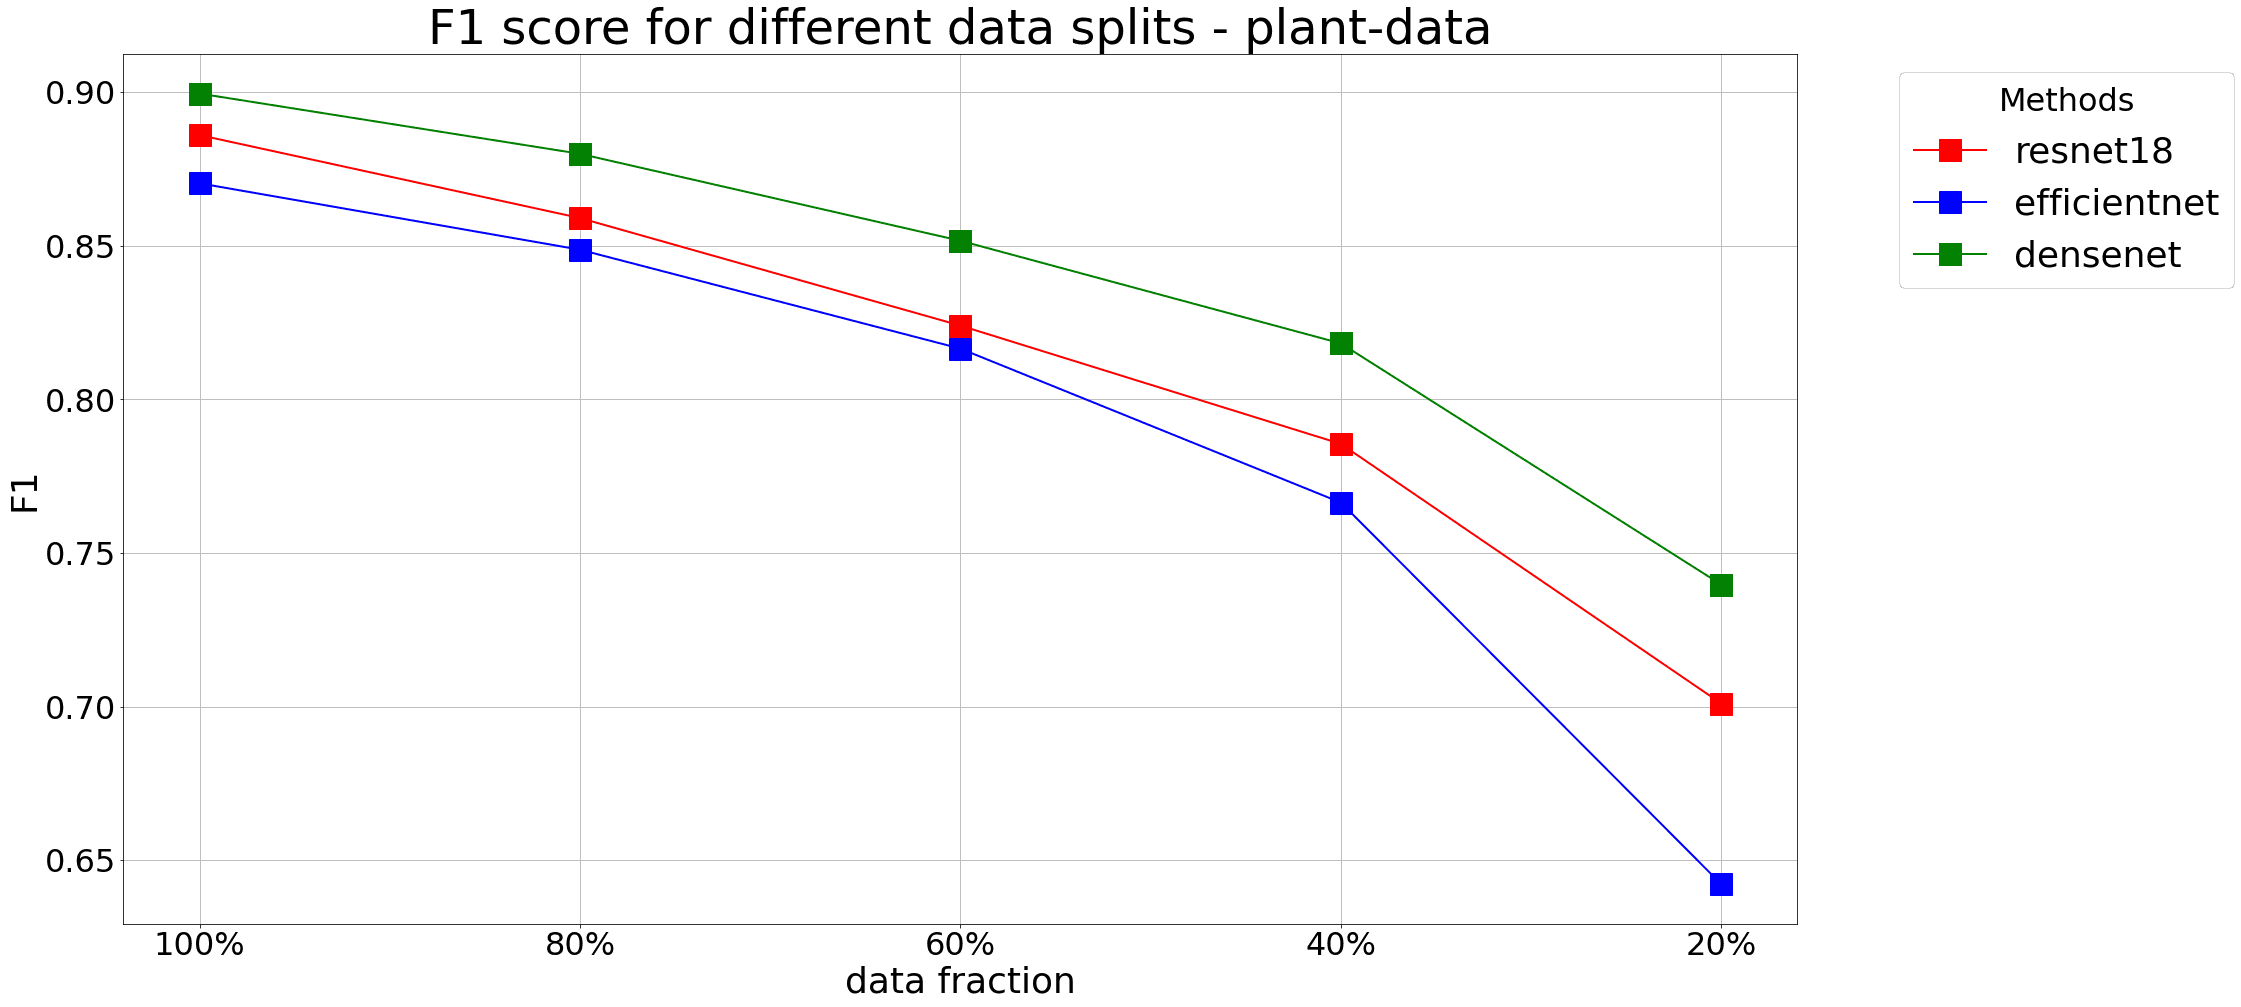
\includegraphics[width=\textwidth]{experiments/models/plant-data-f1.png}
    \caption{Plants dataset, F1 scores}\label{fig:model-scores-plants}
\end{subfigure}

 \caption{F1 scores achieved by models. Each model was trained using a different fraction of the train dataset and then tested on the full test dataset. We can see a significant drop in the models' performance in most of the datasets. The only outliers are visible in models trained on the \textit{Marvel Heroes} dataset (Fig. \ref{fig:model-scores-marvel}), where scores achieved by the models trained on less data are better in two cases.}\label{fig:model-scores}
\end{figure}

\vspace{\baselineskip}

The results of the training process are aligned with the assumption made (remark \ref{remark:performance-drop-while-train}). Models' performance drops with removing more and more data from the training dataset. There are three exceptions, and all of them are related to the Marvel dataset (see Fig. \ref{fig:model-scores-marvel}). All the architectures observed a slight increase of models' score when were trained on less than $100\%$ of the training dataset. That increase did not last when more data was removed, and the rest of the datasets (Fig. \ref{fig:model-scores-dogs}, Fig. \ref{fig:model-scores-food101}, Fig. \ref{fig:model-scores-edible-plants}, Fig. \ref{fig:model-scores-plants}) did not experience the same phenomenon. Detail results are available in appendix \ref{appendix:models:scores}.